\section{Model}


\subsection{Machine Learning}

One of the earliest research about medication names detection in social media was conducted by Jimeno-Yepes et al.~\cite{jimeno2015identifying}. They used two off-the-shelf classifiers - MetaMap~\footnote{\url{https://metamap.nlm.nih.gov/}}, and the Stanford NER tagger~\footnote{\url{https://nlp.stanford.edu/software/CRF-NER.html}}, and a method based on conditional random fields. Jonnagaddala et al.~\cite{jonnagaddala2016binary}, as a part of PSB 2016 Social Media Mining shared task ~\footnote{\url{http://diego.asu.edu/psb2016/task2data.html}}, developed a methodology using SVM to classify whether tweets contains ADR or not. Sarker et al.~\cite{sarker2016social} proposed a stacking based ensemble classifier to automatically detect whether tweets are medication abuse or not for specific 4 medications. The architecture of the methodology is shown in Figure~\ref{fig:model-sarker}. In the ensemble classifier, they used four algorithms - naive bayes (NB), SVM, maximum entropy (ME), and J48, and used various features such as n-gram, abuse-indicating terms, lexicon matches, synonym expansion, word cloud. They concluded that tweets are often ambiguous and impersonal, and a large number of corpus needed for better results. A sample of their annotated data is available~\footnote{\url{http://diego.asu.edu/Publications/DrugAbuse_DrugSafety.html}}. Meanwhile, Zhang et al.~\cite{zhang2016ensemble} applied an ensemble algorithm of four classifiers to detect a tweet contains ADR or not: (1) a concept-matching classifier based on ADR lexicon; (2) a ME classifier with word-level n-gram features and TFIDF weighting scheme; (3) a ME classifier based on word-level n-grams using NB log count ratios as feature values; and (4) a ME classifier with word embedding features. The code of their model is available~\footnote{\url{https://github.com/tjflexic/psb-adr}}. Dai et al.~\cite{dai2016feature} applied SVM to classify ADR posts and features such as linguistic, polarity, lexicon, and topic modeling based features. The resources applied for this research is available~\footnote{\url{https://sites.google.com/site/hjdairesearch/Projects/adverse-drug-reaction-mining}}. Alimova et al.~\cite{alimova2017automated} applied two types of feature engineering(context-level and entity-level) and applied two machine learning based models - Linear SVM and Logistic Regression (LR). The source code of this model is available~\footnote{\url{https://github.com/Ilseyar/adr_classification}}.

\begin{figure}[h]
	\centering
	\begin{minipage}{0.45\textwidth}
		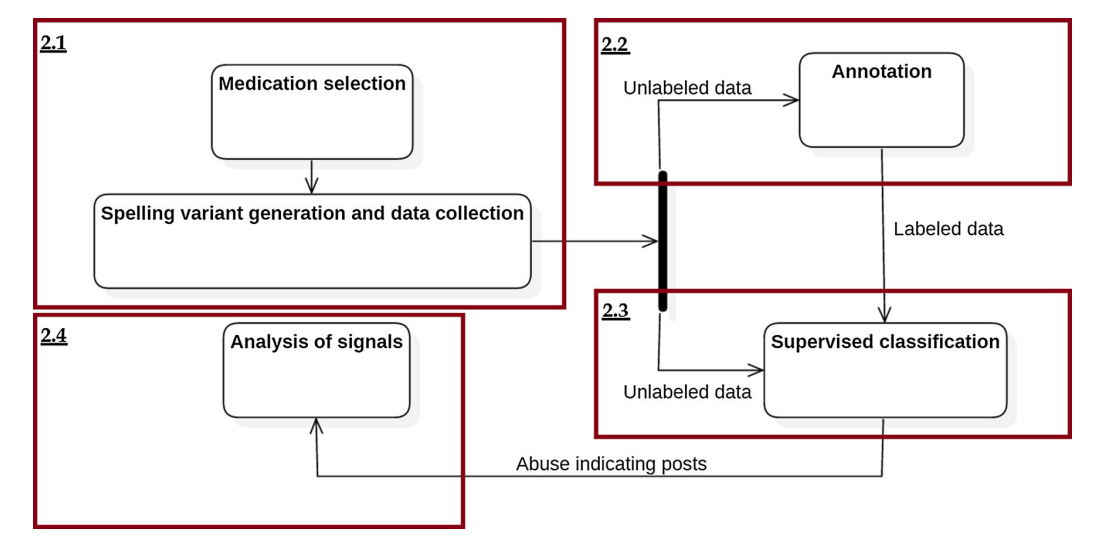
\includegraphics[width=0.99\linewidth]{Figures/h.png}
		\caption{Architecture by Sarker et al.~\cite{sarker2016social}}
		\label{fig:model-sarker}
	\end{minipage}
	\hfill
	\begin{minipage}{0.45\textwidth}
		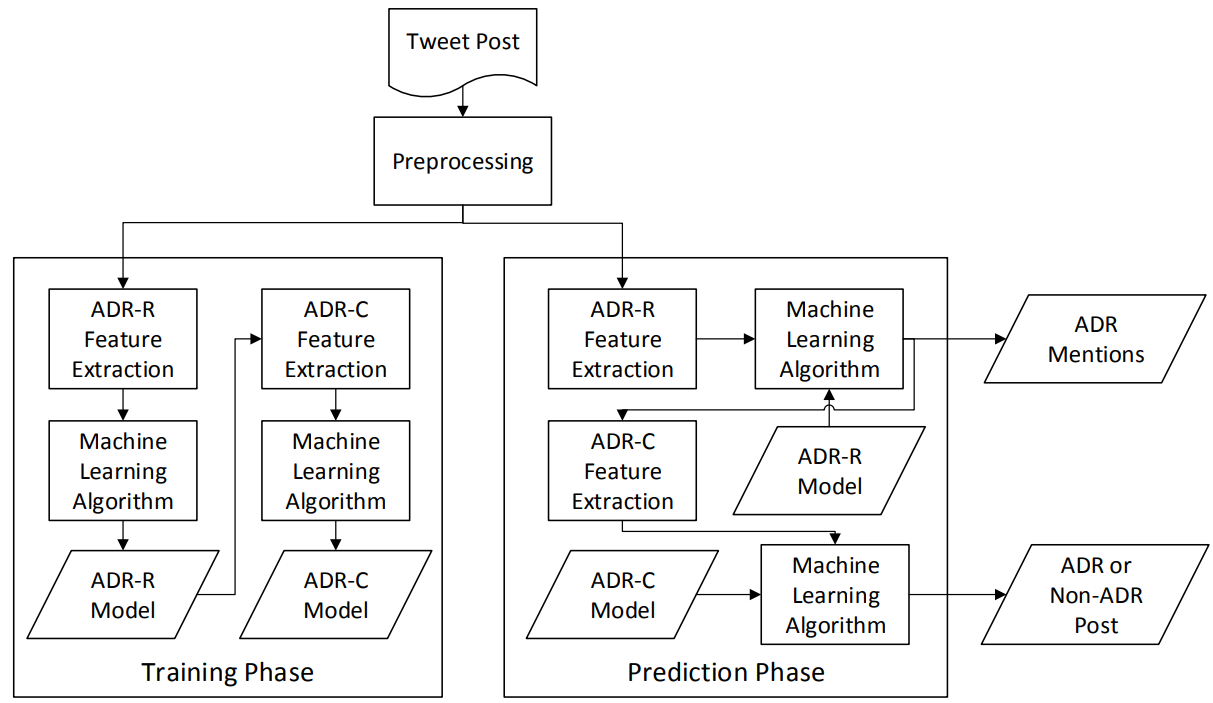
\includegraphics[width=0.99\linewidth]{Figures/r.png}
		\caption{Flow chart of Dai et al.~\cite{dai2016feature}’s methodology.}
		\label{fig:flowchart-alvaro}
	\end{minipage}
\end{figure}


These machine learning based approaches~\cite{jonnagaddala2016binary, sarker2016social, zhang2016ensemble, dai2016feature, alimova2017automated} heavily rely on feature engineering and require large amount of expert knowledge.

\subsection{Deep Learning}

Recently the focus has shifted towards deep learning. Tutubalina et al.~\cite{TUTUBALINA201893} proposed a model based on bidirectional RNN for MCN in social media. The architecture is illustrated in Figure~\ref{fig:architecture-tutubalina}. Huynh et al.~\cite{huynh2016adverse} investigated different neural network (NN) architecture for ADR classification. In particular, they applied their data over four algorithms: CNN, Recurrent Convolutional Neural Network (RCNN), Convolutional Recurrent Neural Network (CRNN), Convolutional Neural Network with Attention (CNNA). The architecture of these algorithms are shown in the Figure 7. The source code of the project is available~\footnote{\url{https://github.com/trunghlt/AdverseDrugReaction}}. Lee et al.~\cite{lee2017adverse}, meanwhile, applied a semi-supervised CNN framework for the same task. This model was developed by Johnson et al.~\cite{johnson2015semi}. Lee proposed a Semi-supervised CNN model. The architecture of the model is shown in the Figure~\ref{fig:architecture-lee}. The method works in two phases: (1) unsupervised phrase embedding learning, and (2) integrating the learned embeddings into the supervised training that uses labeled data. Wu et al.~\cite{wu2018detecting, wu2019msa} proposed neural approach using multi-head self-attention (MSA) to jointly detect drug name and adverse drug reaction. Their MSA model has three modules: first, a word representation module, which aims to build the contextual representations of words from the original characters within them; second, a tweet representation module; third, a classification module. The framework of the model is illustrated in the Figure~\ref{fig:architecture-wu-msa}.

\begin{figure}[h]
	\centering
	\begin{minipage}{0.45\textwidth}
		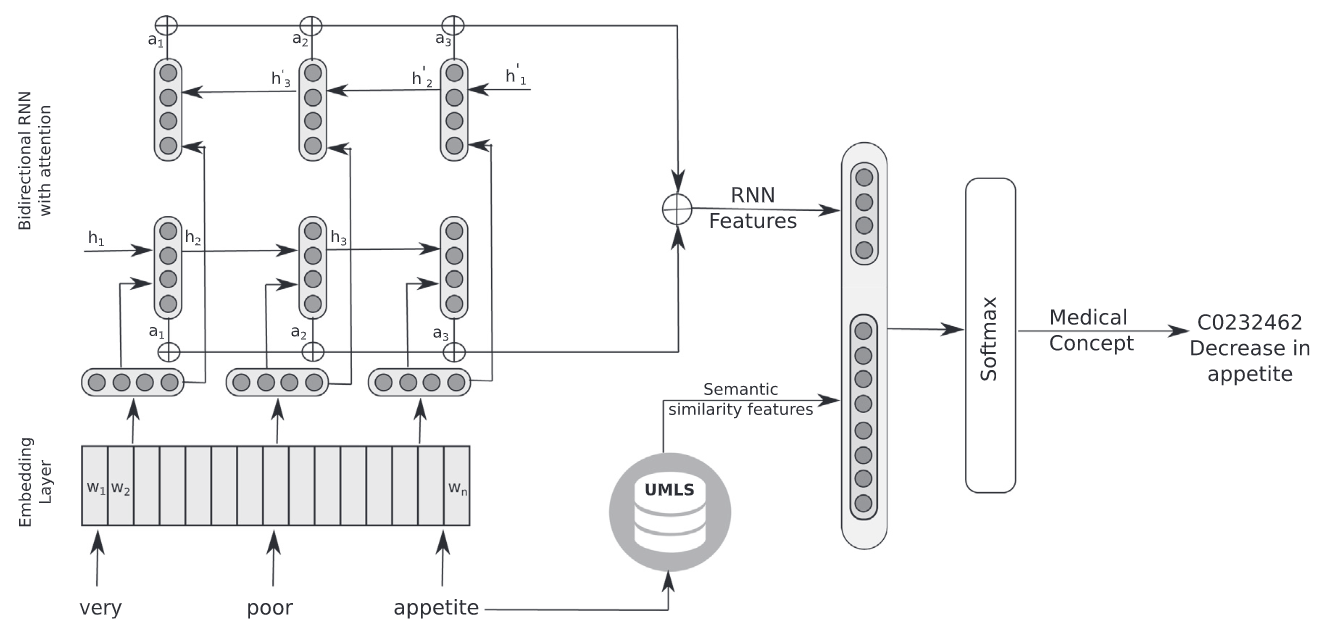
\includegraphics[width=0.99\linewidth]{Figures/f.png}
		\caption{Architecture for MCN in social media by Tutubalina et al.~\cite{TUTUBALINA201893}.}
		\label{fig:architecture-tutubalina}
	\end{minipage}
	\hfill
	\begin{minipage}{0.45\textwidth}
		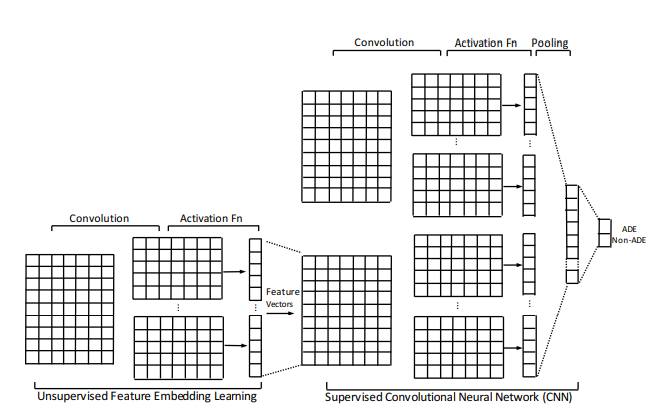
\includegraphics[width=0.99\linewidth]{Figures/l.png}
		\caption{Semi-supervised CNN by Lee et al.~\cite{lee2017adverse}.}
		\label{fig:architecture-lee}
	\end{minipage}
\end{figure}

\begin{figure}[h]
	\centering
	\begin{minipage}{0.45\textwidth}
		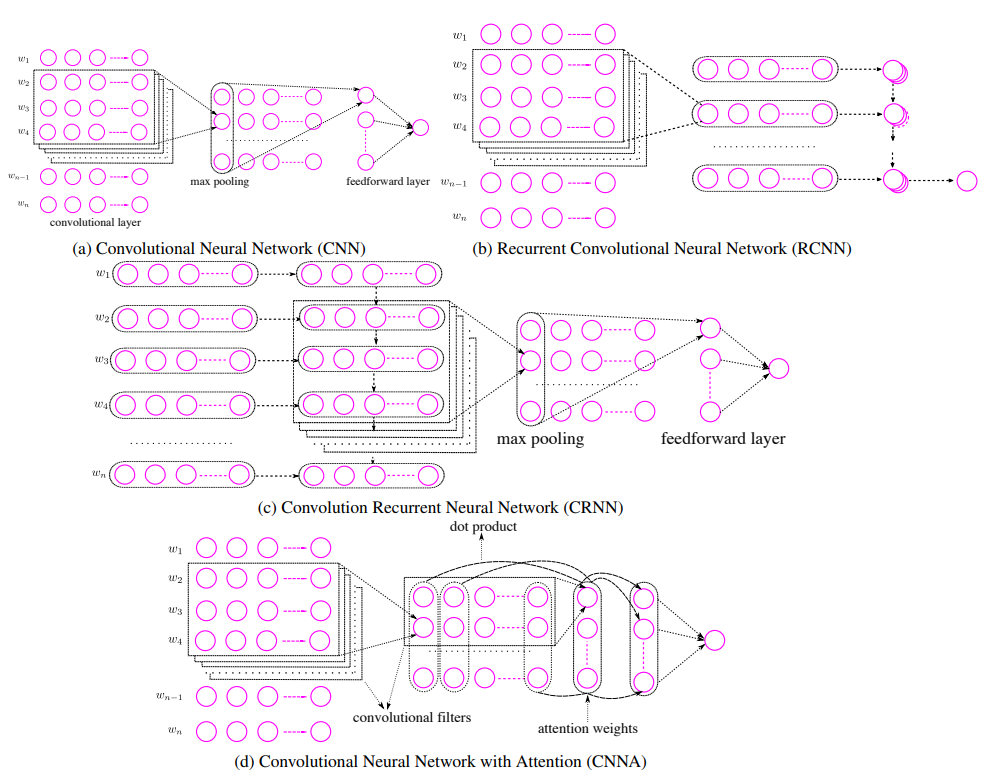
\includegraphics[width=0.99\linewidth]{Figures/e.png}
		\caption{Architecture by Huynh et al.~\cite{huynh2016adverse}.}
		\label{fig:architecture-huynh}		
	\end{minipage}
	\hfill
	\begin{minipage}{0.45\textwidth}
		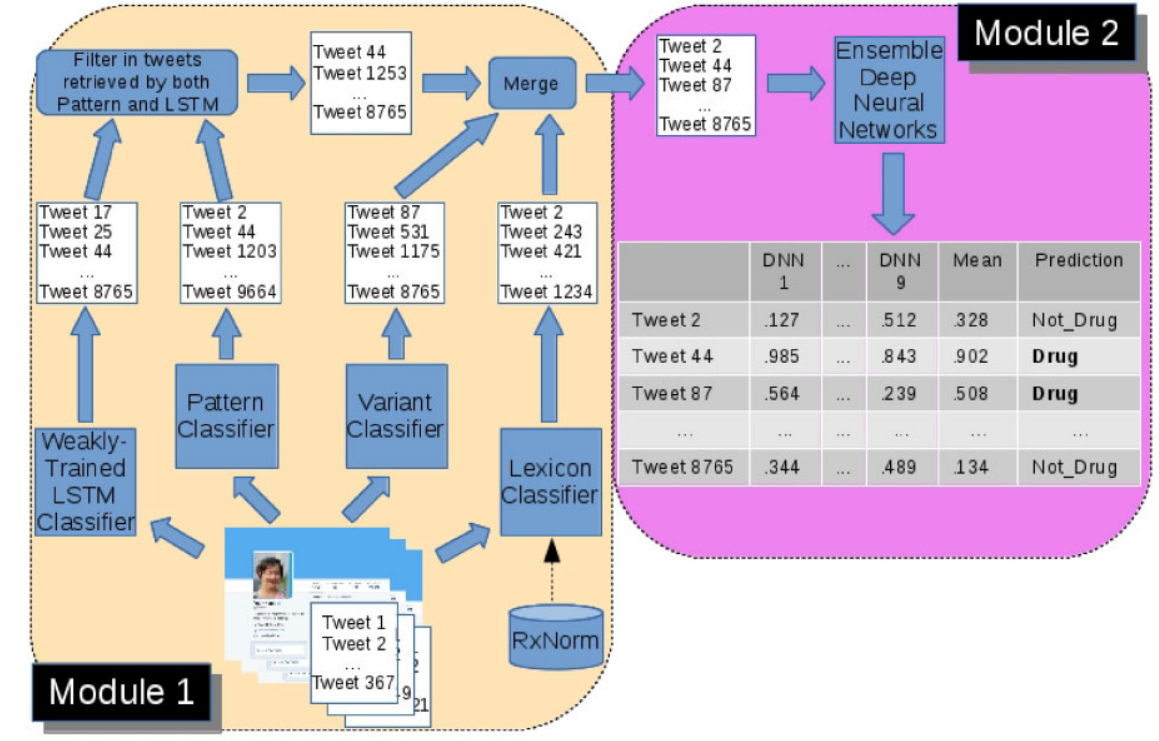
\includegraphics[width=0.99\linewidth]{Figures/a.png}
		\caption{\textit{Kusuri} model by Weissenbacher et al.~\cite{weissenbacher2019deep}.}
		\label{fig:architecture-weissenbacher}
	\end{minipage}
\end{figure}


Weissenbacher et al.~\cite{weissenbacher2019deep} introduced a deep neural networks ensemble method - \textit{Kusuri} - a LSTM model - to detect medication names in unbalanced tweets. \textit{Kusuri} is composed of two modules: first, applied four different classifiers (lexicon based, spelling variant based, pattern based, and a weakly trained neural network) parallel to discover potential tweets with medication names; second, an ensemble of deep neural networks encoding morphological, semantic, and longrange dependencies of important words in the tweets makes the final decision. The architecture is shown in Figure~\ref{fig:architecture-weissenbacher}. A brief description of four algorithms are provided by the authors~\footnote{\url{https://tinyurl.com/y47qzbcq}}. 

\begin{figure}[h]
	\centering
	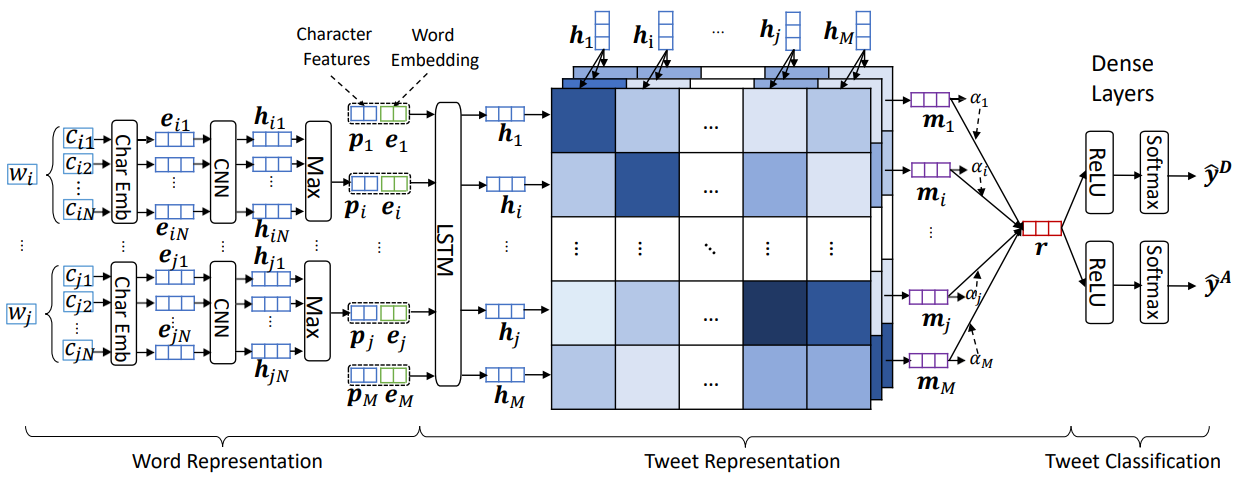
\includegraphics[width=0.99\linewidth]{Figures/k.png}
	\caption{MSA model by Wu et al.~\cite{wu2019msa, wu2018detecting}.}
	\label{fig:architecture-wu-msa} 
\end{figure}

Both supervised and unsupervised models have been developed based on neural networks architecture. CNN~\cite{wu2019msa, huynh2016adverse, lee2017adverse} and RNN~\cite{TUTUBALINA201893, huynh2016adverse} based models have been popular among researchers.